 \section{Introduction}
%Asynchronous message passing is a prevalent programming model in high performance computing (HPC). The model consists of two operations, send and receive, that are essential to message communication. The message communication is complicated because of the non-determinism that a receive may be matched with more than one send in the runtime. The use of match pair, a pair of a send and a receive that may potentially match in the runtime, is able to capture the message communication.
%The semantics can also be complicated because of two buffering settings in the runtime, infinite buffer (messages are buffered in the system) and zero buffer (no buffering in the system). Further, typical message passing standard such as message passing interface (MPI) specifies a special communication that uses collective operations to synchronize a program leading to a more complex program behavior. 
%Given the semantics, several common problems exist in message passing applications: the user-provided assertion may be violated in an execution; the program may deadlock for unexpected matching of receives; and the program may be incompatible with zero buffer semantics, meaning that no feasible schedule exists under zero buffer setting. 
Asynchronous message passing is a prevalent programming model in high performance computing (HPC).
The idea of message passing is simple at the outset: processes communicate within a single node or among multi-nodes by sending messages from one to another. It does not take long, however, to realize that despite the simplicity of the programming model, there is a lot of subtlety in message passing that can impact program behavior. For example, depending on the library, a programmer must be aware of such things as message non-determinism (concurrent sends to a process can arrive in any order), buffering semantics in the runtime (a process may block if the buffer is full), or broad synchronization operations that message with  groups of processes at the same time (i.e., collective operations). This inherent complexity means that the problems of determining if a message passing program is free of deadlock, compatible with a given buffering semantics, or if the message non-determinism affects the correctness of the computation are all NP-complete. %\cite{DBLP:conf/fm/ForejtKNS14}. 
Witnessing any of these properties for an input program is hard.

Prior works on program correctness in the message passing paradigm can be roughly grouped into several approaches. Runtime verification observes the program execution but does not manipulate the execution \cite{DBLP:conf/sc/VetterS00,DBLP:conf/parco/KrammerBMR03,DBLP:conf/ptw/HilbrichSSM09}. The approach is efficient in error detection, but is not precise for reasoning about message non-determinism. Model checking, in contrast, provides precision in analysis as a model of the original program is fully analyzed \cite{DBLP:conf/vmcai/Siegel07,DBLP:conf/pvm/Siegel07}. However, model checking suffers from the state space explosion problem making it unable to analyze large, complex programs. Dynamic analysis greatly improves efficiency by avoiding to explore a large set of non-feasible scheduling outcomes, but is still hard to scale to large, complex programs, especially when there is a high degree of message non-determinism \cite{DBLP:conf/ppopp/VakkalankaSGK08,DBLP:conf/sbmf/SharmaGB12}. 
Symbolic model checking is most possible to provide both precision and efficiency for large programs because the program behavior is highly abstracted in a symbolic encoding which can be quickly analyzed by the state-of-the-art SMT solver \cite{DBLP:conf/kbse/HuangMM13,HuangNFM15,DBLP:conf/fm/ForejtKNS14,DBLP:journals/toplas/ForejtJKNS17}. Thus, this paper looks specifically at symbolic model checking and ways to better leverage the SMT solver in witnessing program properties for message passing programs.

\begin{comment}
dynamic analysis where an existing runtime is manipulated to explore different scheduling outcomes \cite{DBLP:conf/ppopp/VakkalankaSGK08,DBLP:conf/sbmf/SharmaGB12}, model checking where a model of the original program is analyzed \cite{DBLP:conf/vmcai/Siegel07,DBLP:conf/pvm/Siegel07}, runtime verification where the program execution is observed but not manipulated \cite{DBLP:conf/sc/VetterS00,DBLP:conf/parco/KrammerBMR03,DBLP:conf/ptw/HilbrichSSM09}, and symbolic model checking where a model of the program is symbolically analyzed with a Satisfiability modulo theories (SMT) solver \cite{DBLP:conf/kbse/HuangMM13,HuangNFM15,DBLP:conf/fm/ForejtKNS14}. 
%Rebuttal:Review #1.2.2
Generally, runtime verification is efficient in error detection for large programs, but cannot provide precise analysis for message non-determinism. 
Model checking, in contrast, is precise in analysis but suffers from the state space explosion problem. 
Dynamic analysis greatly improves the efficiency compare to model checking, but is still hard to scale to large, complex programs, especially when there is a high degree of message non-determinism.
Symbolic model checking, however, is most possible to provide both precision and efficiency for large programs because the program behavior is highly abstracted in an SMT encoding and the state-of-the-art SMT solver is able to resolve the encoding very quickly.
%Rebuttal
Thus, this paper looks specifically at symbolic model checking and ways to better leverage the SMT solver in witnessing program properties for message passing programs.
\end{comment}

\begin{figure}[h]
\centering
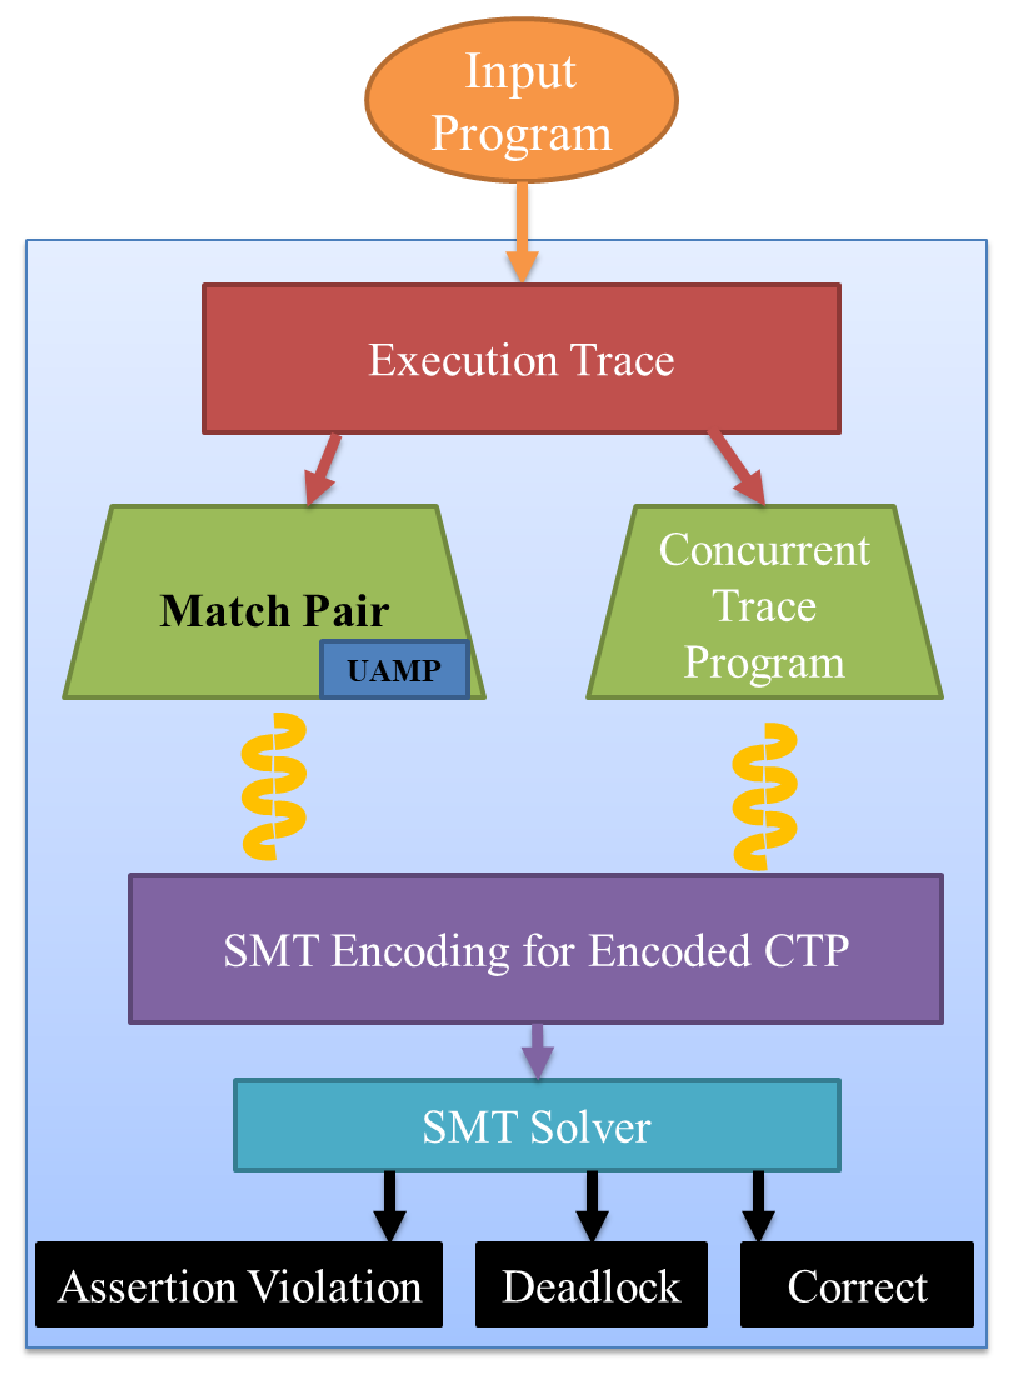
\includegraphics[scale=0.35]{fig/FD.eps}
\caption{Main Framework of Symbolic Model Checking}
\label{fig:framework}
\end{figure}

The general framework of symbolic model checking this paper targets is illustrated in \figref{fig:framework}.
The most efficient types of encoding for symbolic model checking, where efficient means they scale to programs with a high degree of message non-determinism, rely on the concept of a \textit{match pair} and a \textit{concurrent trace program} abstraction (CTP) \cite{DBLP:conf/fmcad/SharmaGMH09,DBLP:conf/sigsoft/WangCGY09}.
A match pair is a send and receive pair that may be matched by the runtime in a feasible program execution. %\cite{DBLP:conf/kbse/HuangMM13,HuangNFM15,deadlock-draft,DBLP:conf/fm/ForejtKNS14,DBLP:conf/atva/ElwakilYW10,DBLP:conf/issta/ElwakilY10}. 
A CTP is an abstraction of the program that removes all branching so each process is a sequence of send, receive, wait (e.g., a witness to the match of a send or receive) and collective operation. %\cite{DBLP:conf/kbse/HuangMM13,HuangNFM15}. 
The abstraction is constructed by observing an execution of the input program for a given input. 
%Therefore, the total number of sends directed to a process is equal to the number of receives in the same process. 
The construction is processed in the runtime of single node or multi-nodes. The message passing standard such as MPI \cite{mpi3.1} does not treat inter-node communication and intra-node communication differently. In other words, the semantics of send-receive matches in a program execution are applicable for both communications. 
Therefore, the match pairs for a CTP are independent of node environments. 
%The approach in this paper is applicable for both environments.
%Once the CTP is constructed, it is further encoded into a set of SMT formulas.
Symbolic model checking gives the SMT solver an encoded CTP with a set of match pairs, and the solver then tries to select a subset of the given match pairs in such a way that the CTP deadlocks or violates an assertion. 

%Rebuttal # 3.2
The SMT solver is efficient for resolving the communication in a CTP rather than the complete behavior in the original program because only the message non-determinism is needed for analysis. The other structures such as branches, loops and different program inputs are ignored in the abstraction of CTP.
However, that does not mean the CTP analysis in this paper only covers a small subset of program behavior.
The symbolic model checking in this paper is extended to exercise, as best as possible, all program behaviors with interesting properties. These behaviors are covered by running the symbolic model checking trace by trace for the target program with respect to a set of test inputs. Each of these tests observes a trace that should be analyzed for deadlock, zero buffer compatibility or assertion violation. The rest of the paper assumes these aforementioned properties.

%To handle the behaviors that may miss from a CTP, the symbolic model checking works trace by trace for the target program with respect to a set of test inputs that intended to exercise, as best as possible, all program behaviors with interesting properties. 
%Each of these tests observes a trace that should be analyzed for deadlock or assertion violation. The rest of the paper assumes these aforementioned properties.
%Rebuttal

%The symbolic model checking requires a over-approximated set of match pairs as input. The set includes all the true match pairs and maybe a few match pairs that may never occur in the runtime. 
%The work then encodes the CTP into an SMT problem that uses a set of formulas to constrain the program behavior based on the semantics. The typical error such as deadlock, zero buffer incompatibility or assertion violation is then checked by solving the SMT problem. If a satisfying assignment exists for the SMT problem, then the error is detected where the match pairs are resolved to capture the message communication in a feasible program execution. If the SMT problem is unsatisfiable, the CTP is free of that error because no feasible schedule exists with any resolution of the match pairs. 

Besides the use of CTP, the input match pair set is more significant for the time cost of symbolic model checking. 
A large input set typically means an expensive SMT solver call especially if there is a high-degree of message non-determinism. 
The idea in this paper is to reduce the cost of the solver call by reducing the size of the input match set to each call. 
Such a reduction cannot, however, be done trivially; any match pair set must be \textit{message complete}.  
A message complete match pair set for a CTP is one that lets the program run to completion (assuming it is free of deadlock). 

%Rebuttal #3.1
To achieve message completion, collective operations must be carefully treated as they can synchronize the program execution thus interrupts with send-receive matches. 
However, reasoning about collective operations with match pair generation is extremely inefficient because an exhaustive exploration of the program behavior is needed. 
Therefore, this paper simply ignores collective operations in match pair generation and is able to include all the match pairs needed for resolving the feasible schedules with collective communication. 
In addition, the collective operations are explicitly encoded by symbolic model checking. As such, the SMT solver is able to automatically pick up the feasible match pairs from the generated ones such that the encoded collective communication is resolved.

%the message complete property also requires that the match pair set is sufficient such that all those interrupted by collective operations in any feasible execution are included.
%The SMT encoding with such a match pair set further constrains the behavior of how collective operations impacts the message passing.
%the collective operations are matched as expected, especially when they interrupts with actual send-receive matches in an execution. 
%Rebuttal

%As such, reducing the size of the input match pair set directly impacts the run time cost, typically, of the SMT solver. A straightforward idea to improve the performance, therefore, is to reduce the number of the match pairs. A naive way of reducing the match pairs such as randomly selecting a subset of the match pairs, however, is not sufficient. The input set of match pairs must be sufficient to complete the message communication in a program execution if the CTP is free of deadlock. A match pair set that has this property for a given CTP is termed \emph{message complete}.
%The input match pairs must satisfy two properties: program completion (the program can run to completion assuming no deadlocks exist) and message non-determinism (the set has a certain degree of non-determinism such that a receive may be associated with more than one match pairs).  
%The algorithm in this paper explores a way to generate such a reduced set of match pairs.

To reduce the number of match pairs and to fulfill the requirement of message completion, this paper describes the under-approximation algorithm for match pair (UAMP). The algorithm successively generates under-approximations of the true set of match pairs until all match pairs are generated. The under-approximations retain the message complete property. 
The symbolic model checking with UAMP focuses on property witnessing rather than proofs of correctness as the intent is to witness program properties early in the iterations before the set of match pairs gets large.
%Since the correctness of a CTP can not be proved given an under-approximated set of match pairs, this paper only discusses the capability of error detection for the SMT encoding. 
%The primary goal is to improve bug finding in a CTP; although, since the algorithm is iterative, it is able to eventually produce a set of match pairs that includes all reachable match pairs in the CTP, therefore it proves correctness. 


Generally, UAMP generates the match pairs in two steps. 
First, each process is sectioned, where a section contains a sequence of receives that are projected from the process and a number of sends from all the senders that may potentially match these receives. 
The number of sends from each sender to a section is roughly bounded by $k$ given as a user input. Note that the value of $k$ determines the number of sections divided by the algorithm. In precise, a larger value of $k$ yields a smaller number of sections, and vice versa. The sends from each sender to the section are distributed sequentially.  
%Here, ``roughly" in the context implies three situations: a sender distributes exactly $k$ sends to the destination section if there are sufficient sends from the sender; the sender distributes less than $k$ sends to the section if either there are insufficient sends from the sender or . 
%For each section, the algorithm precisely adds a set of sequences of sends from multiple potential sender processes.  
The number of receives that are added to the sections is equal to the number of the sends distributed to the section. %Therefore, the number of receives in the section is roughly $k\times n$, where $n$ is the number of available senders.
%The number of the receives depends on three values that are statically known: the positive integer $k$ configured by the user, the number of all the potential sender processes and the number of the unmatched receives in the process. 
Match pairs are then generated for each section independently. 
This independent sectioning effectively ignores combinations of match pairs, that are feasible, but only available when the considered concurrent outstanding sends are more than the number of receives in the section. As such, UAMP has the flexibility to generate the match pair set with various size based on the user input.
UAMP generates the match pairs for the sends and receives in each section by a list of simple rules based on ranks \cite{DBLP:conf/kbse/HuangMM13}. A rank is a non-negative integer that represents the position of a send or a receive in a specific sequence in the section.

%Rebuttal #3.1
%The algorithm is able to identify all potential match pairs in each single section, thus follows the message complete property; the match pairs that are needed for matching all sends and receives in the section with the interruption of collective operations are all included in the generated match pair set. 
%Rebuttal

Given the steps for match pair generation, UAMP starts with $k=1$ and increments $k$ to a larger bound such that the number of the divided sections is changed, because the match pair generation for the new iteration is only meaningful if each process is sectioned differently. The growth of the size of the match pair set is polynomial as $k$ increases. The program property is then witnessed when $k$ is incremented to a sufficiently large bound; or the process repeats.
%Rebuttal #1.2.1
The first bound $k$ that witnesses a program property in the iterative steps above is called the ``\textit{optimal k}''. 
The steps for reaching the \textit{optimal k} is independent of the configurations of machines and processes once the CTP is generated. The construction of the CTP, though, relies on the concrete execution under a specific runtime environment.  
%Rebuttal


%Have you added the discussion that k jumps by increments greater than 1? Meaning that you move k until the number of sections changes? In many regards, that is what is critical; start with k=1, then move k until the # of sections changes, run the solver, repeat. Is that discussion in the paper?


%The key insight of the solution is that each section is considered independently for match pair generation.  
%The algorithm does not generate the match pair for a send and a receive from two different sections, while in fact the send and the receive may match in the runtime. 
%As a result, the algorithm is able to under-approximate the precise match pairs as input to an SMT problem. 
%Due to the missed match pairs that are derived from matching sends and receives in different sections, the SMT problem may not encode the complete program behavior. However, if the problem is satisfiable, then it is known that a specific error exists for a feasible schedule that is resolved by the encoding. As such, the SMT encoding with a reduced set of match pairs can be used to detect errors. If the problem is, however, unsatisfiable for the under-approximated match pairs, it does not mean that there are provably no errors for any feasible execution in the runtime. It is then necessary to generate a larger set of match pairs by a new input K to capture more behavior for detection.


The paper includes the discussion that the precise match pairs for any CTP can be generated with a sufficiently large bound $k$. 
Experiments further show that the runtime cost of witnessing properties is drastically reduced with the initial setting of $k$ which creates simple problem instances for the SMT solver. 
Experiments also show that the symbolic model checking with UAMP is able to scale to a program that employs a high degree of message non-determinism and/or a high degree of deep communication.
Deep communication in this context means that each sender for a receiver issues a long sequence of sends to the receiver.
The contributions include,
\begin{compactitem}
%Rebuttal: Review #1.4.2
\item the first under-approximation algorithm for effectively reasoning about match pairs in a CTP.
%Rebuttal
%where the size depends on a positive integer $k$ configured by the user,
\item the proof that the precise match pairs for any CTP can be generated by the new algorithm with a sufficiently large bound $k$, and
\item the results from the experiments using a set of benchmarks to demonstrate the improved performance of witnessing program properties.
\end{compactitem}

The rest of the paper is organized as follows: 
Sections 2 presents the definition, the semantics and an example of CTP; Section 3 presents the general algorithm in the paper; Section 4 states that the precise match pairs can be generated; Section 5 gives the experimental results; Section 6 discusses the related work; and Section 7 is the conclusion and future work.
